\chapter{Concept}
\label{cha:methoden}

This chapter briefly presents the current state of mobile navigation with ROS and its limitations. 
This chapter aims to identify the critical areas in which standard mobile robots running ROS lack robustness and autonomy during autonomous mobile navigation. According to these critical areas, requirements are derived from them and prioritized with a risk analysis. 
This chapter proposes how behavior planning can improve the current default systems to meet these requirements. 

\section{Current State}
\subsection{ROS}
The Robot Operating System (ROS) is an open-source middleware for creating robot applications. It is not an operating system (OS) since it needs an underlying OS, mainly Linux-based, to work. 
ROS can handle the communication between different programs (called nodes) with standardized interfaces and network protocols. Nodes can communicate via topics, services, and actions, which differ in their application domain (compare table \ref{tab:ros_interfaces}). 

\begin{table}[ht]
	\caption{ROS Communication Options}
	\label{tab:ros_interfaces}
	\begin{tabular}{ | m{0.15\textwidth} | m{0.2\textwidth}| m{0.35\textwidth} | m{0.2\textwidth}|} 
  	\hline
  	\textbf{Name} & \textbf{Communication Pattern} & \textbf{Area of Use} & \textbf{Cardinality} \\ 
  	\hline
  	Topics & Publisher/ Subscriber & Continuous stream of data e.g. sensor data &  n:m \\ 
  	\hline
  	Services & Request/ Response & Get specific data only once & One service, many clients \\ 
  	\hline
  	Actions & Request/ Response and Publish/ Subscribe & Trigger executing of asynchronous goal-driven processes and receive updates & One action, many clients \\
  	\hline
	\end{tabular}
\end{table}

This design choice makes robotic applications built with ROS highly reusable and interchangeable, allowing developers to integrate foreign libraries more easily into their applications. 
Due to the availability of many high-quality open-source libraries for many different use cases, ROS has become the leading methodology for creating robotic applications in the research environment \cite{quigley2009}. 

With ROS2, the framework received fundamental changes and updates to its architecture and design to gain more acceptance and use in the industry. These changes allow for real-time safety, simpler certification, and security when building industrial applications and products using ROS2 \cite{ros2022}.  

\subsection{Navigation2}
The ROS Navigation2 Stack (Nav2) combines different packages that allow mobile robots to navigate from point A to point B. Navigation2 is the de-facto standard for mobile navigation with a wide range of supported robots. Supported robot types are holonomic, differential-drive, legged, and ackerman (car-like). For the mobile robot to make use of the Nav2 stack, it has to be set up in a certain way to be able to generate plans and execute commands in the right way. Nav2 requires the mobile robot to possess a laser scan or point cloud sensor, an odometry source (such as an IMU or wheel encoders), and a set of transformations for planning and navigation. 
The stack contains tools that save and load occupancy maps, localize the robot, plan paths, execute the path, provide cost maps, build behaviors and execute recoveries \cite{macenski2020}. 

\begin{figure}[ht]
	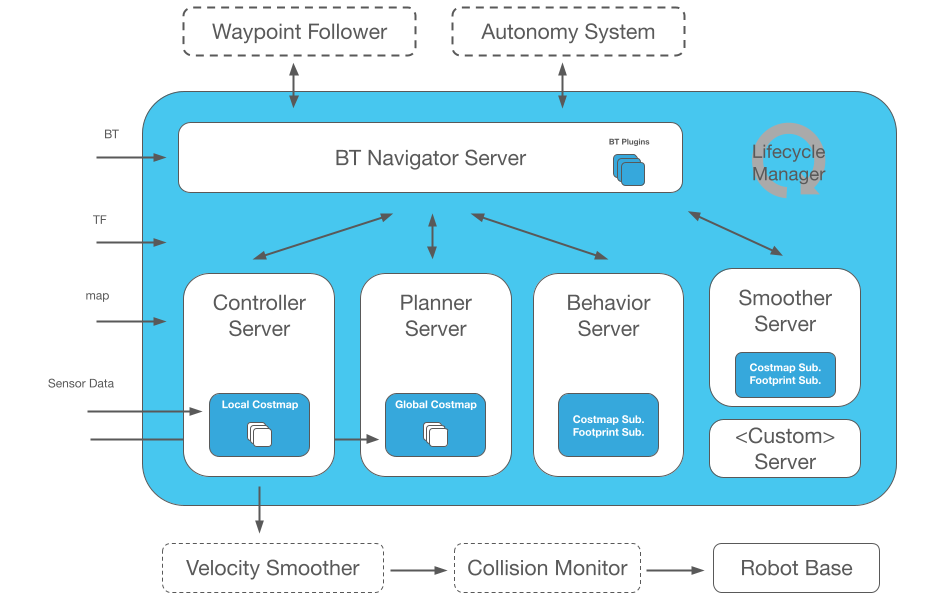
\includegraphics[width=1.0\textwidth]{images/nav2_architecture.png}
	\caption{Navigation2 Architecture \cite{macenski2020}}
	\label{fig:nav_architecture}
\end{figure}
\subparagraph*{}
These packages are often integrating a SLAM method to build or enlarge maps. Path planning and execution capabilities, which correspond to the global and local planner described in section 2.2, are further supported by ready-to-use planning plugins that use A* and Dijkstra algorithms for path planning and a dynamic window approach for path execution. The system sequencing is done in a hierarchical structure as a central behavior tree calls asynchronous actions from the respective planners after another, as seen in figure \ref{fig:nav_architecture}. 

\begin{figure}[ht]
	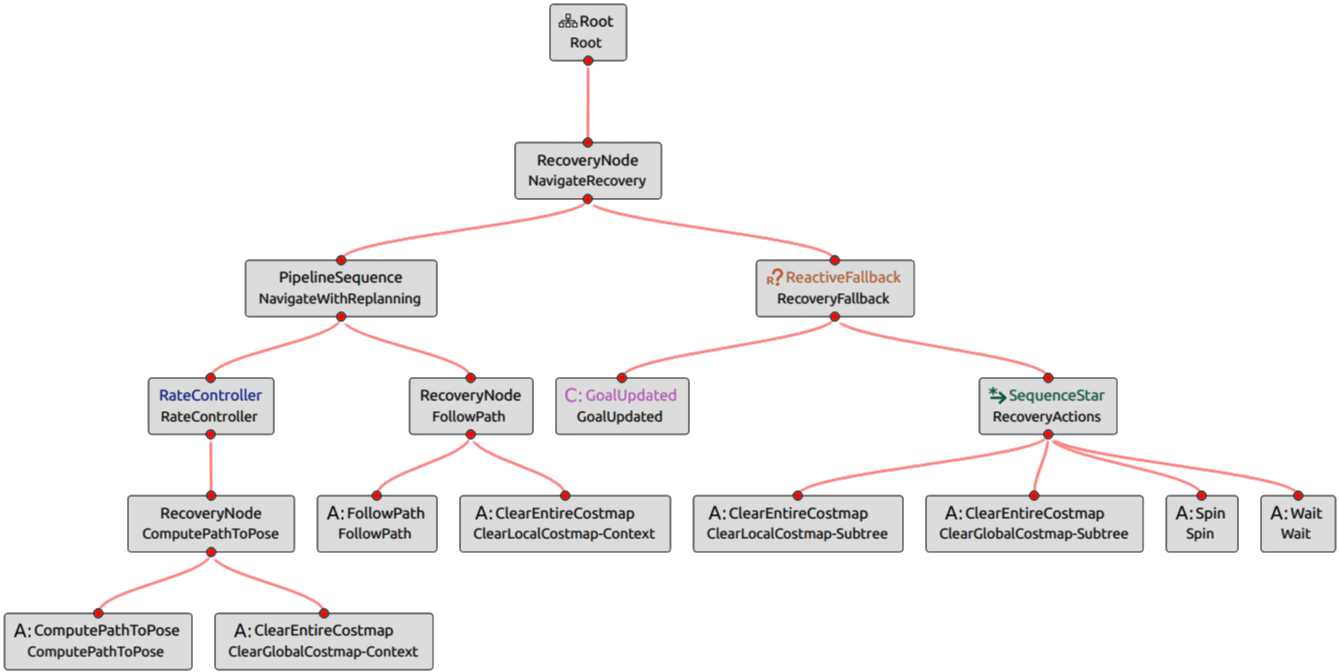
\includegraphics[width=1.0\textwidth]{images/nav_bt-modified.png}
	\caption{Navigation2 Behavior Tree}
	\label{fig:bt_nav}
\end{figure}
\subparagraph*{}
The behavior tree depicted in figure \ref{fig:bt_nav} is the one that is the default Nav2 behavior and has a set of recovery behaviors already implemented (spin, wait, back up, clear map). These behaviors are executed if the robot can not make progress towards the set goal. 
Nav2 uses a node lifecycle management system to start, activate, deactivate, and shut down nodes in a controlled way. The lifecycle approach allows the system degree to monitor the system node's startups, executions, and failures. 
\subparagraph*{}
With this quantity of functions and hierarchical architecture, the ROS Navigation2 stack is an excellent basis for achieving high levels of robot autonomy. The software can be modified and expanded with plugins to fit the users' needs. 
When comparing the functionalities of the software stack to the proposed autonomous system architecture in figure \ref{fig:autonomous_driving_architectures}, the things that Nav2 is missing are a system-wide supervision layer and a more deliberative approach to behavior planning, as mentioned in chapter 2.3.
\subparagraph*{}
The absence of these components leads to a limited set of circumstances in which the robot can perform navigation reliably. One of the core problems behavior-based robots face is generating a dependable environment representation. An accurate representation is the basis for the last steps in the planning part of the "Sense - Think - Act" cycle. Unforeseen events can severely limit the reliability of the environment representation without the robot being aware of it. Examples of such events currently not handled appropriately are slipping wheels, orientation changes by external influences, or undetected, more specifically, undetectable obstacles. 
%\textit{Add statistics about random sensor failures every ~10000h} 
This can lead to erratic movement of the robot, as reactive behaviors and more deliberative behaviors compete for authority over the robot's movement. By design, to allow more intelligent robot behaviors, the deliberative behavior can override commands from reactive behaviors. However, the deliberative behavior's planning is based upon a false representation of reality, leading to unsafe commands. The unsafe planning triggers reactive-type behaviors again to counteract the commands from the deliberative behavior. Even worse would be that the reactive behaviors may not get activated, and the robot continues to drive despite being unaware of the surroundings. The unsafe behavior requires a human operator would need to step in and restore the robot to full functionality by hand. 

%\textit{Add a closing statement about that suitability of the Nav stack for achieving autonomy}


\subsection{Turtlebot3}
The Turtlebot3 is a standard mobile research platform with an available ROS interface to control the robot. The robot is well integrated into the ROS ecosystem and is established in the literature as a system to develop and integrate new methods. 
The robot has two motors with attached wheel encoders to drive and steer, classifying it as a differential drive robot. A third omnidirectional wheel stabilizes the robot. 
\subparagraph*{}
The manufacturer provides an open-source model for simulating the robot in physics-based simulators like Gazebo, as depicted in figure \ref{fig:turtlebot}, which enables faster development and testing for the robot. 
\begin{center}
\begin{figure}[ht]   
	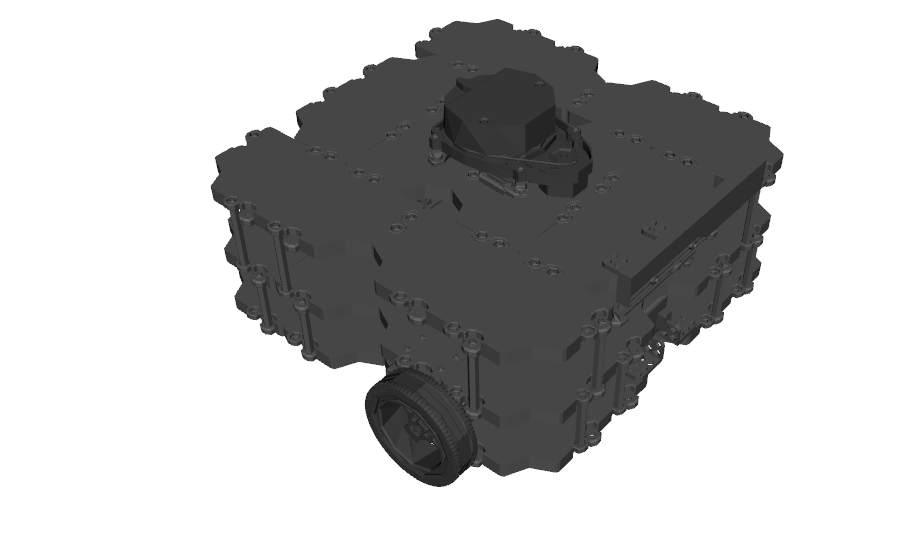
\includegraphics[width=0.7\textwidth]{images/turtlebot_sim.png}
	\caption{Turtlebot3 model in Gazebo simulator}
	\label{fig:turtlebot}
\end{figure}
\end{center}
The equipped sensors and easy simulation capabilities make the robot well suited for using the Nav2 stack and further development for behavior planning. 

The robot specifications are specified in table \ref{tab:turtlebot_spec}. 

\begin{table}[ht]
\caption{Turtlebot3 Specifications}
\label{tab:turtlebot_spec}
	\begin{tabular}{| m{0.3\textwidth} | m{0.3\textwidth} |} 
  	\hline
  	\textbf{Specification} & \textbf{Value} \\ 
  	\hline
  	Maximum translational velocity & 0.26 m/s \\ 
  	\hline
  	Maximum rotational velocity & 1.82 rad/s (104.27 deg/s) \\
  	\hline
  	Maximum payload & 30kg \\
  	\hline
  	Size (L x W x H) & 281mm x 306mm x 141mm \\
  	\hline
  	Weight & 1.8 kg \\
  	\hline
  	Singe Board Computer & Raspberry Pi (3 or 4) \\
  	\hline
  	Laser Distance Sensor & 360 Degree Laser Distance Sensor LDS-01 \\
  	\hline
  	IMU & Gyroscope 3 Axis, Accelerometer 3 Axis \\
  	\hline
  	Actuators & XM430-W210 \\
  	\hline
	\end{tabular}
\end{table}

The turtlebot will be used for the analysis of the current state of mobile navigation. Furthermore, the simulated turtlebot will be the platform on which the behavior planning will be implemented and tested.


\section{Requirements}

The software requirements that improve the robot's behavior are derived from the current limitations of the standard ROS and Navigation2 setup for mobile robots described in the previous chapter. 
The functional requirements and their acceptance criteria are listed in \ref{tab:fn_req}. The non-functional requirements are listed seperately in \ref{tab:nonfn_req}. 
To better contextualize the context of the systems requirements, figure \ref{fig:use_case} depicts a Use-Case diagram with the needed functions to improve the system's autonomy.

\begin{table}[ht]
\caption{Functional Requirements}
\label{tab:fn_req}
	\begin{tabular}{| m{0.08\textwidth} | m{0.13\textwidth}| m{0.09\textwidth} | m{0.60\textwidth}|} 
  	\hline
  	\textbf{Nr.} & \textbf{Name} & \textbf{Priority} & \textbf{Description/Acceptance Criteria} \\ 
  	\hline
  	fn$\_$req1 & Sensor Failure & High & The system detects sensor failure. Ensure that the system can restart sensors and decrease the speed during the time the sensor delivers limited information \\ 
  	\hline
  	fn$\_$req2 & Emergency Detection & High & The system detects emergency. Ensure that the system can detect when the continuation on the calculated path is no longer safe (sensor failures, blockage) \\
  	\hline
  	fn$\_$req3 & Emergency Stop & High & The system can initiate emergency stops. Ensure that the system can override all commands and stop in case an emergency is detected \\
  	\hline  	
  	fn$\_$req4 & Override Navigation2 & High & The system can override navigation2. Ensure that the system's commands can always override the commands coming from navigation2. \\
  	\hline
  	fn$\_$req5 & Maintain operability & High & The robot executes commands as long as it is safe. Ensure that the robot keeps driving if it is safe even when system functions are not working correctly. \\
  	\hline
  	fn$\_$req6 & Recovery & High &  The system can recover from crashes. Ensure that the system can successfully reach goals despite previous crashes\\ 
  	\hline  
  	fn$\_$req7 & Control Path Planning & Medium & The system controls and rates the quality of the planned paths. \\
  	\hline	
  	fn$\_$req8 & Reset Goals & Medium & The system can reset and override goals set by the user so that the goal is reachable by planners. \\
  	\hline
  	fn$\_$req9 & Robot Range & Medium & Ensure that the robot will not run out of battery during navigation to a goal.  \\	
  	\hline
	\end{tabular}
\end{table}


\begin{table}[ht]
	\caption{Non-Functional Requirements}
	\label{tab:nonfn_req}
	\begin{tabular}{ | m{0.13\textwidth} | m{0.13\textwidth}| m{0.1\textwidth} | m{0.55\textwidth} |} 
  	\hline
  	\textbf{Nr.} & \textbf{Name} & \textbf{Priority} & \textbf{Description} \\ 
  	\hline
  	non$\_$freq1 & Single Point of Failure & High &  The system does not have a single point of failure	When parts of the system fail, the system maintains operability to a degree \\ 
  	\hline
  	non$\_$freq2 & Performance & High & The system's control loop guarantees fast reactions. The average frequency with which the system checks the sensors/navigation2 is higher than 100Hz (10ms) \\ 
  	\hline
  	non$\_$freq3 & Determinism & High & The outcome for a given set of inputs must be deterministic, meaning that the behavior is always executed similarly. \\
  	\hline
  	non$\_$freq4 & Deliberate & High & The robot can execute deliberative behaviors, meaning that behaviors new implemented behaviors go beyond reacting to sensor input and have a planning aspect. \\
  	\hline
	\end{tabular}
\end{table}

\begin{figure}[ht]   
	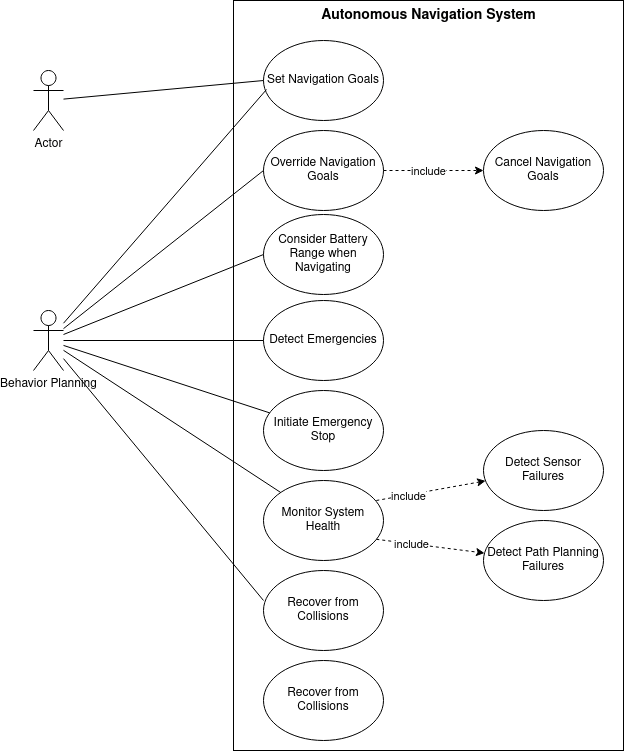
\includegraphics[width=0.7\textwidth]{images/use_case.png}
	\caption{Use Case Diagram}
	\label{fig:use_case}
\end{figure}


\section{System Solution}

For a Turtlebot3 running Nav2 to appropriately deal with the listed requirements, the system needs to be extended with new external modules. To eliminate a single point of failure for the system, one needs to create an independent second system outside the existing one. This is to create a robust fallback behavior that does not rely on Nav2 to move. Also, an external system can more reliably monitor other systems when its execution is detached from the performance and execution of other systems. 
A suitable name for the second system is the "autonomy layer", as it aims to increase the robustness and autonomy of the whole system. 
The autonomy layer has to provide a comprehensive system supervisor that monitors all components' health (sensors, navigation, robot controller). The constant execution monitoring equips the system with the ability to deal with the event of node failures and component malfunctions.
\subparagraph*{}
Another required addition to the autonomy layer is a data storage of relevant system information. The stored data includes sensor data and generated maps, cost maps, positions, and speed commands. Using past data points allows behaviors to become more deliberative in their approach and opens up many possibilities for intelligent behaviors like movement predictions of obstacles. 
\subparagraph*{}
A third component to the autonomy layer is a behavior planner largely independent of Nav2 execution and planning. This behavior planner must be capable of overriding the Nav2 behaviors if needed. The component processes information from the execution checker, Nav2, and past and present sensor data to decide if and how to override the default behaviors. Based on this information, the behavior planner can make a deliberative, strategic decision to increase robustness and autonomy, thus decreasing reliance on human supervision.
\subparagraph*{}
Additionally, a component to switch intelligently between speed commands from Nav2 and the autonomy layer is needed. This component could be realized as a decision gate that receives speed commands from Nav2 and the new behavior planning component and can forward, block or modify commands sent to the controller. This modification aspect allows high-quality local planning capabilities but enables more deliberative behaviors to happen upon this planning. A simplified system block diagram is depicted in figure \ref{fig:block_diagram}. The proposed additional components, discussed in this chapter are colored in blue. Existing components, discussed in chapter 3.1, are colored in gray. 

\begin{center}
\begin{figure}[ht]   
	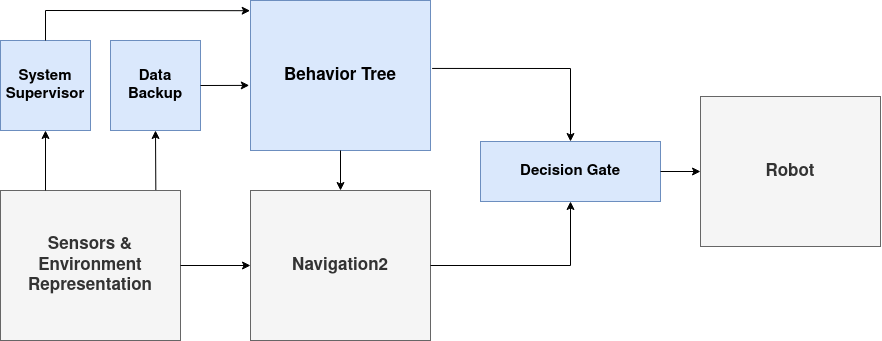
\includegraphics[width=1.0\textwidth]{images/block_diagram.png}
	\caption{System Block Diagram}
	\label{fig:block_diagram}
\end{figure}
\end{center}


\section{Software and Simulation}
A comparison and assessment of the behavior planning approach were made in chapter 2.4. The decision on which approach to take fell on the behavior tree method. The reason for this is mainly the increased flexibility when creating and expanding the behavior planning compared to FSMs. Also, behavior trees allow complete determinism and introspection.
%which is why POMPDs are not suitable as the behavior planning approach for the specified requirements. 

\subsection{Behaviortree.CPP}
The Navigation2 stack uses a behavior tree to coordinate the planning layer. The behavior tree that is used is an expansion of the Behaviortree.CPP (BT.CPP) library. This library offers a fast way to create, execute, monitor, and edit behavior trees. 
Additionally to the types of control nodes that are mentioned in chapter 2.4.2, the library adds the concept of reactivity into the catalog of control nodes. Reactive sequences and reactive fallbacks differ from normal ones in handling nodes that return the state "running". Instead of ticking the node again, the whole sequence restarts, which is very useful for continuously checking a condition and executing an asynchronous action node that gets halted when a condition is not met anymore (compare table \ref{tab:control_nodes_bt}). 

\begin{table}[ht]
	\caption{Control Nodes in BT.CPP}
	\label{tab:control_nodes_bt}
	\begin{tabular}{ | m{0.2\textwidth} | m{0.25\textwidth}| m{0.25\textwidth} | m{0.2\textwidth} |} 
  	\hline
  	\textbf{Name }& \textbf{Child returns Failure} & \textbf{Child Returns Running} \\ 
  	\hline
  	Sequence & Restart & Tick Again\\ 
  	\hline
  	Reactive Sequence & Restart & Restart \\ 
  	\hline
  	Sequence Star & Tick again & Tick again \\
  	\hline
  	Fallback & Tick next & Tick again\\
  	\hline  	
  	Reactive Fallback & Tick next & Restart \\
  	\hline
	\end{tabular}
\end{table}

Also, it offers Decorator Nodes which allow more control over the child node and its output. These Decorator Nodes can only have one child node each. A comprehensive list of the available Decorators and descriptions is presented in table \ref{tab:decorators_bt}.

\begin{center}
\begin{table}[ht]
	\caption{Decorator Nodes in BT.CPP}
	\label{tab:decorators_bt}
	\begin{tabular}{ | m{0.2\textwidth} | m{0.25\textwidth}| m{0.25\textwidth} | m{0.2\textwidth} |} 
  	\hline
  	\textbf{Name} & \textbf{Succeeds} & \textbf{Fails} & \textbf{Running} \\ 
  	\hline
  	Inverter Node & If the child returns false & If child return success &  If the child returns running \\ 
  	\hline
  	ForceSuccess Node & Always & Never & If child returns running \\ 
  	\hline
  	ForceFailure Node & Never & Always & If child returns running\\
  	\hline
  	Repeat Node & Ticks child as long as it returns success. The maximum number of repeats can be defined & If the child returns failure & If the child returns running \\
  	\hline  	
  	Retry Node & If the child returns success & Ticks child as long as it returns failure. The maximum number of ticks can be defined & If the child returns running. \\
  	\hline
	\end{tabular}
\end{table}
\end{center}

\subparagraph*{}
To allow the tree nodes to communicate, the library provides the developer with two possibilities. Either node can use the blackboard, a dictionary (key/value) that all nodes of the tree can read and write. Alternatively, two nodes can be connected through ports which allows direct communication between two nodes via a key/value.

\subsection{Groot}

Groot is a software to create, edit, monitor, and debug behavior trees with a graphical user interface. The software allows the creation of behavior trees in XML files which can be directly loaded into and used by the BT.CPP library. Groot can monitor the live execution of behavior trees and allows the introspection of how the tree reacts to different scenarios.

%\textit{Screenshot of live monitoring}

\subsection{Gazebo Simulation Environment}
The development and testing of behaviors will be done with the Gazebo simulator and the Turtlebot3 model. Gazebo is well-integrated into ROS and ROS2 and offers many ROS interfaces to control the simulation. Gazebo accurately models the physics of the robot and can simulate and publish the wheel odometry directly on a ROS topic. Furthermore, the simulator can simulate the readings for the laser scanner and IMU data via plugins. The use of the simulator allows easier repeatability for test cases as various obstacles can be spawned at any time, and sensor failures can be easily induced, resulting in quicker overall development.
Using a simulator allows slowing down or speeding up the environment time. The time control allows more intricate observation of fast reactive type behaviors in slow motion while also enabling the observation of the long-time robustness of the system during extended tests. 
The ROS community offers many different simulation environments to test the robot in. The environments range from simple geometric structurs, to office spaces up to complete race tracks. 

\subsection{OS and Software Versions}
The software versions used to implment and test the system on are listed below in table \ref{tab:versions}. Many of the software versions are determined by the choice of the ROS distribution (distro). ROS2 Foxy is not the newest ROS2 distribution but is well supported and developed, so the decision was made to use this distribution. The decision why the turtlebot is used is laid out in chapter 3.1.3. Although Python and C++ can be used to develop applications with ROS2, the behavior tree library relies on C++, which is why C++ was used for developing the whole system. 

\begin{center}
\begin{table}[ht]
	\caption{Decorator Nodes in BT.CPP}
	\label{tab:versions}
	\begin{tabular}{ | m{0.2\textwidth} | m{0.25\textwidth}| m{0.25\textwidth} | m{0.2\textwidth} |} 
  	\hline
  	\textbf{Name} & \textbf{Version / Release} & \textbf{Comments} \\ 
  	\hline
  	Operating System & Ubuntu 20.04 LTS &  \\ 
  	\hline
  	ROS & ROS2 Foxy & Long-Term-Supported Distribution \\ 
  	\hline
  	Navigation2 & Foxy-devel & Newest Release for ROS2 Foxy\\
  	\hline
  	Simulation & Gazebo 11 & Determined by choice of ROS Distro \\
  	\hline  	
  	Robot & Turtlebot3 &  \\
  	\hline
  	Behavior Tree & BT.CPP 3.7 & \\
  	\hline
  	Programming Language & C++ 14 & Determined by choice of ROS Distro \\
  	\hline
  	Build System & CMake and Colcon & Determined by choice of ROS Distro \\
  	\hline
  	Development Environment & Visual Studio Code & Offers IDE debugging options for ROS \\
  	\hline
	\end{tabular}
\end{table}
\end{center}
